\subsubsection{UC20 - Modifica file di configurazione del dizionario dati}\label{UC20}

\begin{figure}[H]
  \centering
  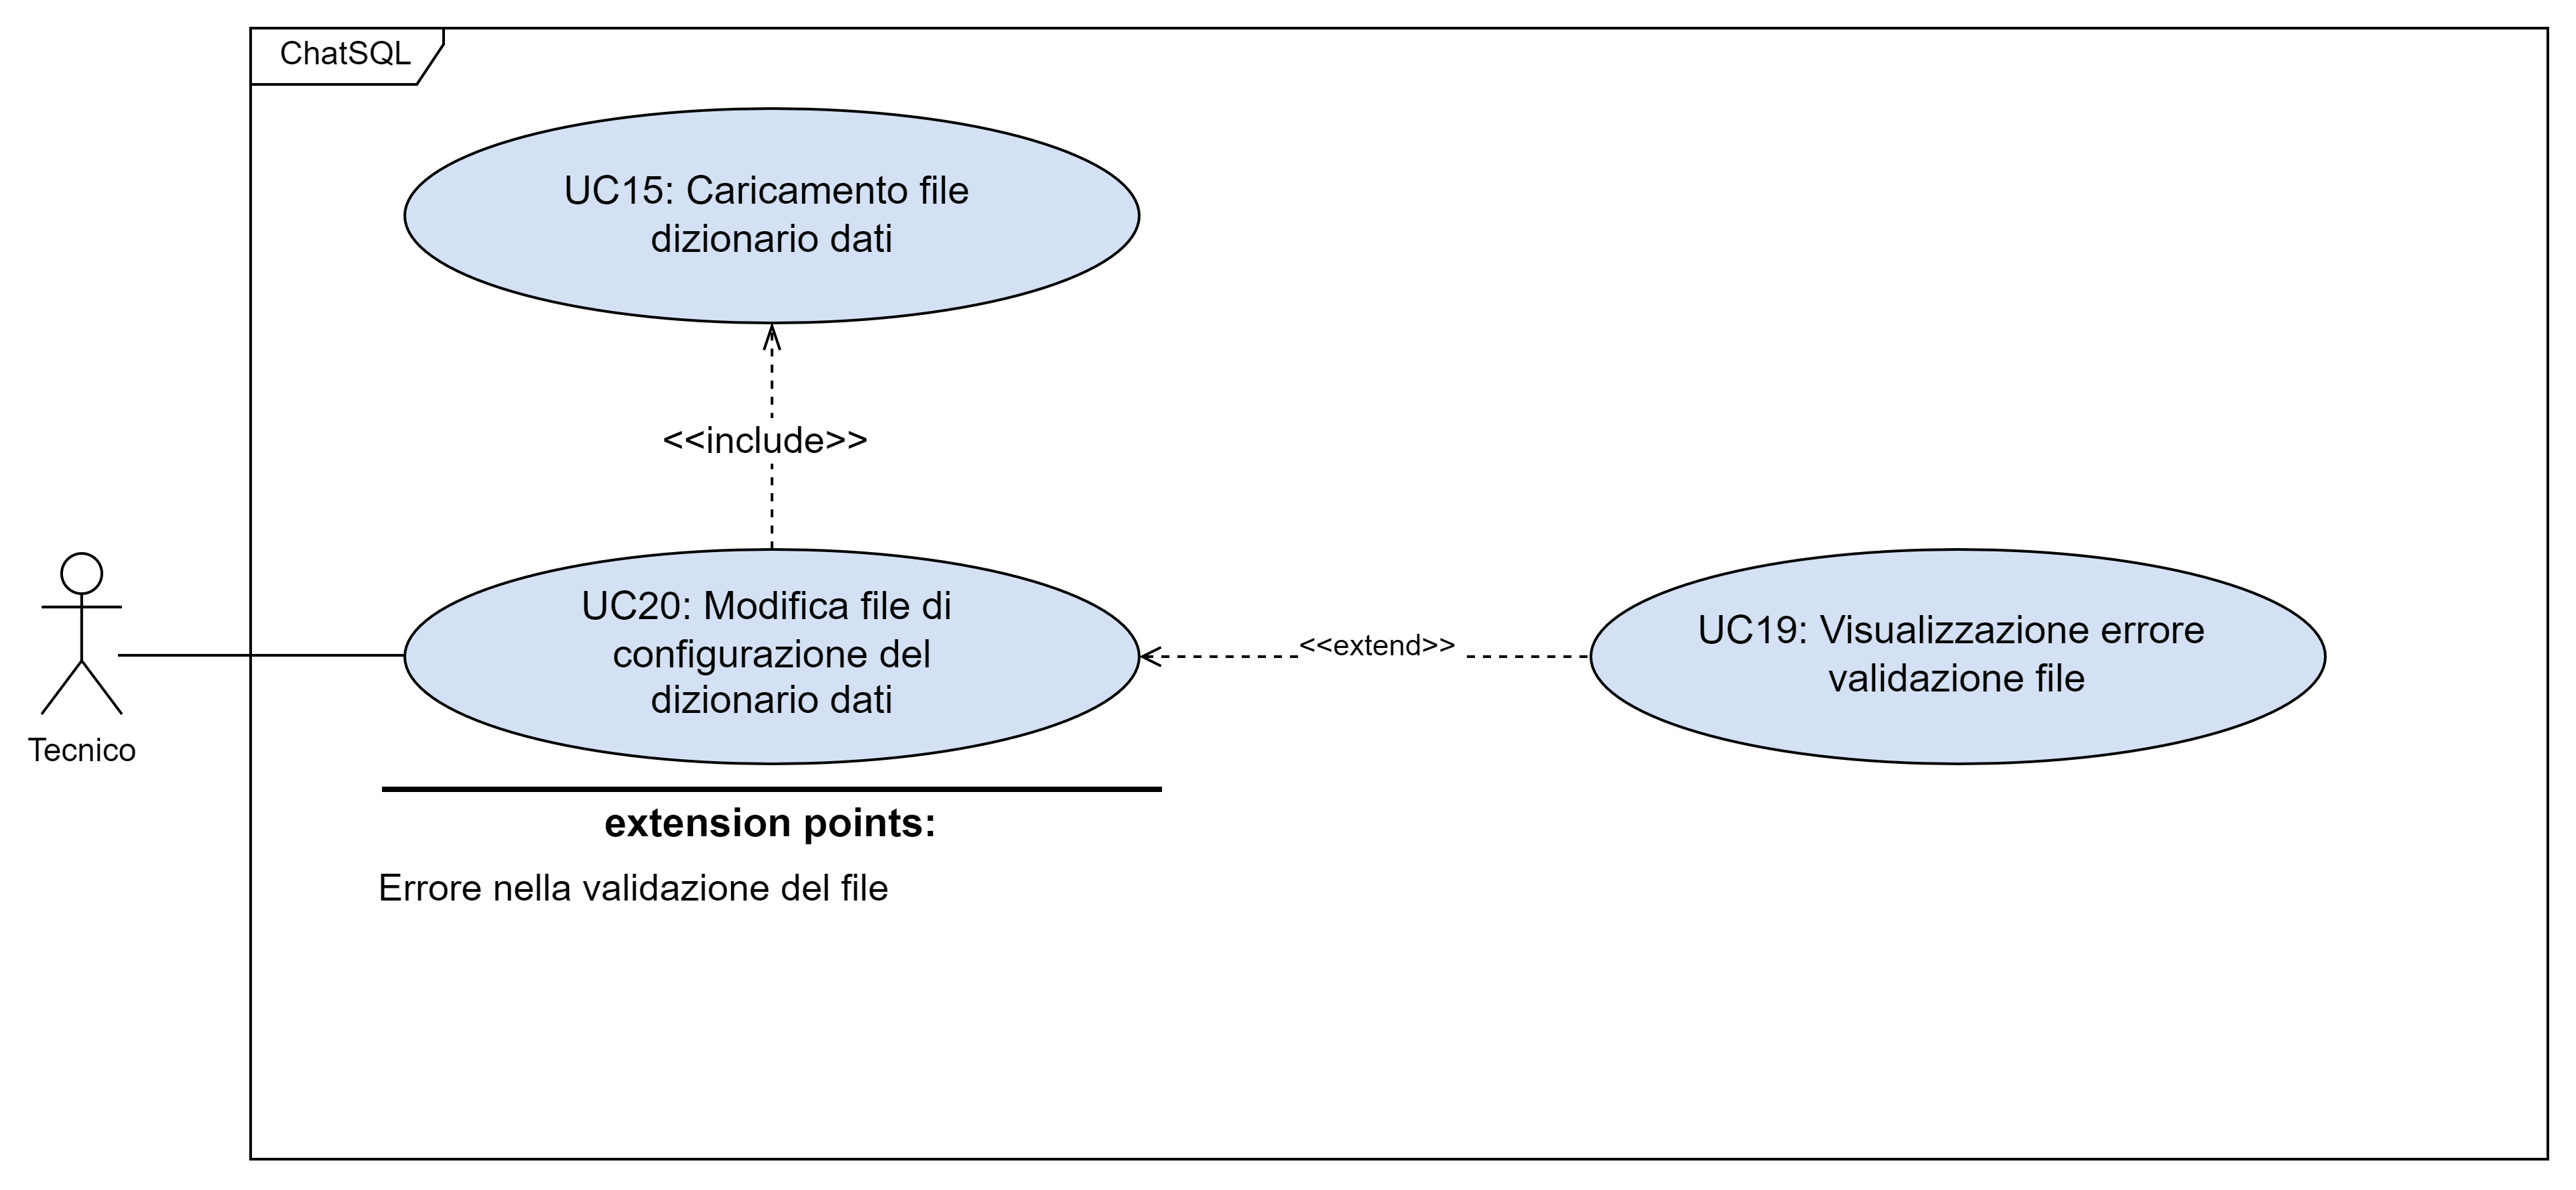
\includegraphics[width=0.95\textwidth]{assets/uc20.png}
  \caption{UC20}
\end{figure}

\paragraph*{Descrizione}
Il Tecnico modifica il file di configurazione di un \glossario{dizionario dati}. Con il termine file di configurazione si intende il file che contiene la descrizione del database in formato strutturato. 

\paragraph*{Attori principali}
Tecnico

\paragraph*{Precondizioni}
\begin{itemize}
  \item Il sistema è attivo e funzionante;
  \item Il Tecnico ha effettuato l'autenticazione (\hyperref[UC1]{UC1});
  \item Il Tecnico ha visualizzato la lista dei \glossario{dizionari dati} (\hyperref[UC9]{UC9});
  \item Il Tecnico ha individuato il dizionario da modificare (\hyperref[UC9.1]{UC9.1}).
\end{itemize}

\paragraph*{Postcondizioni}
\begin{itemize}
  \item Il file di configurazione del \glossario{dizionario dati} è stato sostituito correttamente.
\end{itemize}

\paragraph*{Trigger}
Il Tecnico vuole modificare il file di configurazione di un \glossario{dizionario dati}.

\paragraph*{Scenario principale}
\begin{enumerate}
  \item Il Tecnico avvia la procedura di modifica di un \glossario{dizionario dati};
  \item Il Tecnico inserisce un nuovo file;
  \item Il Tecnico richiede il salvataggio del file;
  \item Il sistema sovrascrive il file precedentemente caricato.
\end{enumerate}

\paragraph*{Scenario alternativo}
\begin{enumerate}
  \item Il sistema riscontra un errore nella validazione del file (\hyperref[UC19]{UC19});
  \item Viene visualizzato un messaggio con i dettagli dell'errore.
\end{enumerate}

\paragraph*{Inclusioni}
\begin{itemize}
  \item Caricamento file \glossario{dizionario dati} (\hyperref[UC15]{UC15}).
\end{itemize}

\paragraph*{Estensioni}
\begin{itemize}
  \item Visualizzazione errore validazione file (\hyperref[UC19]{UC19}):
  \begin{itemize}
    \item Extension point: Errore nella validazione del file;
    \item Condition: Formato del file non valido, file troppo pesante, file non conforme allo schema predefinito.
  \end{itemize}
\end{itemize}